\section{Introduction}
\label{sec:whitepaper_introduction}

For over a decade, \textit{wireless sensor networks} (WSNs) fostered the
development of new applications and trends in the broad areas of mobile
and opportunistic computing. Such networks are composed of multiple small,
low-cost and low-power, multipurpose sensor nodes that communicate with
each other over small distances using the wireless medium
\cite{culler:2004}. Their \textit{self-organizing} capabilities, due to
their ad hoc communication paradigm, make them suitable for deployment on
demand. This saves engineering time, reduces the installation costs, and
accommodates the ad hoc deployment of a wireless network during disaster
emergencies or military operations. Hence, applications of WSNs are
pervasive in military (\textit{e.g.,} ammunition monitoring, battlefield
surveillance, sniper localization \cite{simon:2004}, reconnaissance,
damage assessment), environment (\textit{e.g.,} animal tracking
\cite{szewczyk:2004}, chemical detection \cite{allred:2007}, pollution
monitoring \cite{hartung:2006}), health (\textit{e.g.,} patient
monitoring and drug surveillance in hospitals) \cite{lorincz:2008}, home
automation (\textit{e.g.,} ``smart home'') \cite{kim:2008}, as well as in
the commercial domain (\textit{e.g.,} monitoring construction material,
inventory management, building automation, vehicle tracking).

Figure~\ref{fig:mote_arch} illustrates the architectural components of a
typical sensor node (also known as ``mote''). Each mote consists of a
\textit{micro-controller}, an outward \textit{power source}, a
\textit{transceiver}, some amount of \textit{external memory}
(\textit{i.e.,} external in terms of the micro-controller), and a set of
\textit{sensor devices} all connected with the micro-controller through an
\textit{analog-to-digital converter} (ADC). Each node senses its external
environment and conveys the perceived data to nearby nodes using the IEEE
802.15.4 wireless communication standard. Moreover, special purpose nodes
act as \textit{base stations} and collect all sensor data in order to
further deliver them to aggregation points. That is, they act as
``bridges'' between network boundaries, or help in establishing a
multi-tier network topology \cite{gnawali:2006}.

\begin{figure}[htp]
\centering
	\includegraphics[scale=0.7]{fig/mote_arch.eps}
	\caption{Sensor node (\textit{mote}) architecture.}
	\label{fig:mote_arch}
\end{figure}

In the early 2000's, WSNs were envisioned as the materialization of the
``Smart Dust'' concept (\textit{i.e.,} millimeter scale sensing and
communication platforms) \cite{smartdust}. However, due to power
consumption issues we have yet to witnesses nodes of such scale; instead
of ``dust'' sensors, we had only sensors at the size of a small PDA.
Having said that, recent advances on the sensor chips exploit
\textit{ambient} power (\textit{e.g.,} radio power from the TV and FM
radio) in order to further miniaturize their size by avoiding batteries.
Moreover, they offer accurate estimates of the processing that can be
performed with certain amount of consumable energy, fueling even more the 
development of new services of \textit{ubiquitous} manner. As a
characteristic example consider the Central Nervous System for the Earth 
(CeNSE) project, which has been announced by HP and aims at the
development of trillion nano-scale sensors and actuators that will all be
interconnected with computing systems and provide new services
\cite{cense}.


\section{Problem Statement}

Akyildiz \textit{et al.,} \cite{wsn_survey} surveyed a large number of
different WSN applications and identified a set of factors that affect 
the design of a sensor network. Such factors include fault tolerance,
scalability, operating environment, network topology, hardware
constraints, transmission media, and various others. This variety of
aspects that deeply affect the design, and therefore the implementation
and operation, of a WSN, gave rise to an enormous number of WSN
applications that heavily re-implement basic system facilities
(\textit{e.g.,} network protocols, routing, data dissemination and
collection) in order to provide optimal results. This style of development
although it offers many degrees of freedom for the design and development 
of new and elaborate facilities, it has also serious drawbacks; it delays 
the adoption of the WSN technology by non-experts (\textit{i.e.,} a
typical vendor that provides WSN software and services should have deep
understanding and expertise in various fields, ranging from OS development
to routing protocol design and implementation). 

Fennec Fox is a platform that facilitates policy-based, self-controlling,
dynamic network \textit{reconfiguration} of low-power and lossy networks
(\textit{e.g.,} WSNs). It aims at maximizing the efficiency of the system
by managing the provided resources, appropriately, so as to meed
application requirements at the lowest possible cost. The WSN operation
is constrained by power, memory, and computational resources. Sensor nodes
are typically battery powered, with few kB to few MB of memory, and have
limited processing power (\textit{e.g.,} their clock speed ranges from kHz
to few MHz). Using these limited resources, WSNs are expected to support
various applications. The Fennec Fox platform is the apparatus of a
philosophy, which assumes that WSN applications consist of a \textit{chain
of network tasks}.

A task is defined as a simple computational operation, optimized to
perform some functionality given certain constraints (\textit{e.g.,} power
consumption, delay, security). During their life-cycle, Fennec Fox-based
sensor nodes \textit{transition} between various states, where each state
performs a simple task. In this context, applications running on Fennec
Fox identify conditions for transitioning between various tasks, and
controlling the behavior of the tasks, by specifying task parameters.
However, to perform their job, tasks require support from other parts of
the WSN that provide various services, such as routing or sensing.
Therefore, sensor states are not only represented by the task which they
perform, but also by a set of other WSN systems that help this task to
achieve its expected results. 

Fennec Fox was motivated by the need to \textit{auto-configure},
\textit{reprogram}, and \textit{manage} wireless sensor networks. Since
such tasks are already complicated by themselves, Fennec Fox attempts also
to simplify the modeling and programming of sensornets. That is,
sensornets are required to auto-configure themselves during their lifetime.
\footnote{Ali El Kateeb has stated that ``because wireless sensor network
applications are new and might require abilities not fully anticipated
during design and development, supporting sensor networks with
design-modification capabilities is vital to making sensor-network
platforms capable of adjusting to their surrounding environment after
initial network deployments.'' \cite{kateeb:2009}}

Fennec Fox is built out of three logical components: 
a \textit{dynamic network stack}, a \textit{policy control unit}, and a
\textit{user programmable application layer}. The dynamic network stack is
a library, consisting of protocols and utilities for providing a high
level abstraction to the TinyOS \cite{hill:2000} system, which supports
adaptive applications. Policy control unit is the component responsible
for guiding the transitioning between different stack configurations. 
The transitions are expressed in form of policies, which in response to an
event, reconfigure the stack. Finally, the application layer provides a
simplified API; it allows the programmer to focus on the application logic,
instead of reprogramming communication protocols or mathematical functions.
Swift Fox language is a high-level ``handle'' for programming Fennec Fox.
The following example demonstrates the usage of Fennec Fox and Swift Fox
and defines their relationship. Suppose that we have a WSN for home
monitoring that is also capable of handling emergency situations. In this
setup, our network application supports two scenarios; the first one is
focusing on monitoring the home environment by collecting sample data
from all sensor nodes, and the second one is focusing on monitoring areas
with the potential of fire. For the needs of the second scenario, the WSN
is capable of taking and streaming pictures. Yet, collecting sensor data,
such as light intensity, humidity, and temperature, requires network
protocols that can support the type of network traffic generated by sensor 
nodes, as well as a network topology that can efficiently disseminate the
collected data. A simple representation of data collection scenario is
illustrated on Figure \ref{fig:scenarioa}. In the second scenario, the
sensors detect a fire, based on multi-modal correlation of sensor readings
that represent increased probability of fire occurrence. In that case, when
fire is detected, we want the system to capture pictures of the fire area
to verify the correctness of the fire alert and also as estimate if there
are still people around the fire area who can be in danger.

From the network communication perspective, this scenario requires
establishing \textit{point-to-point} communication between a sensor node,
which can capture a picture of the area in fire, and the sink node, for 
providing direct high bandwidth communication for data transmission in an
emergency situation such as this one. A representation of network
configuration supporting this scenario is shown in Figure
\ref{fig:scenariob}. Both figures show scenarios with different data flow
objectives: \textit{network energy conservation} versus \textit{low-delay
direct data transmission}. 

\begin{figure}
\centering
	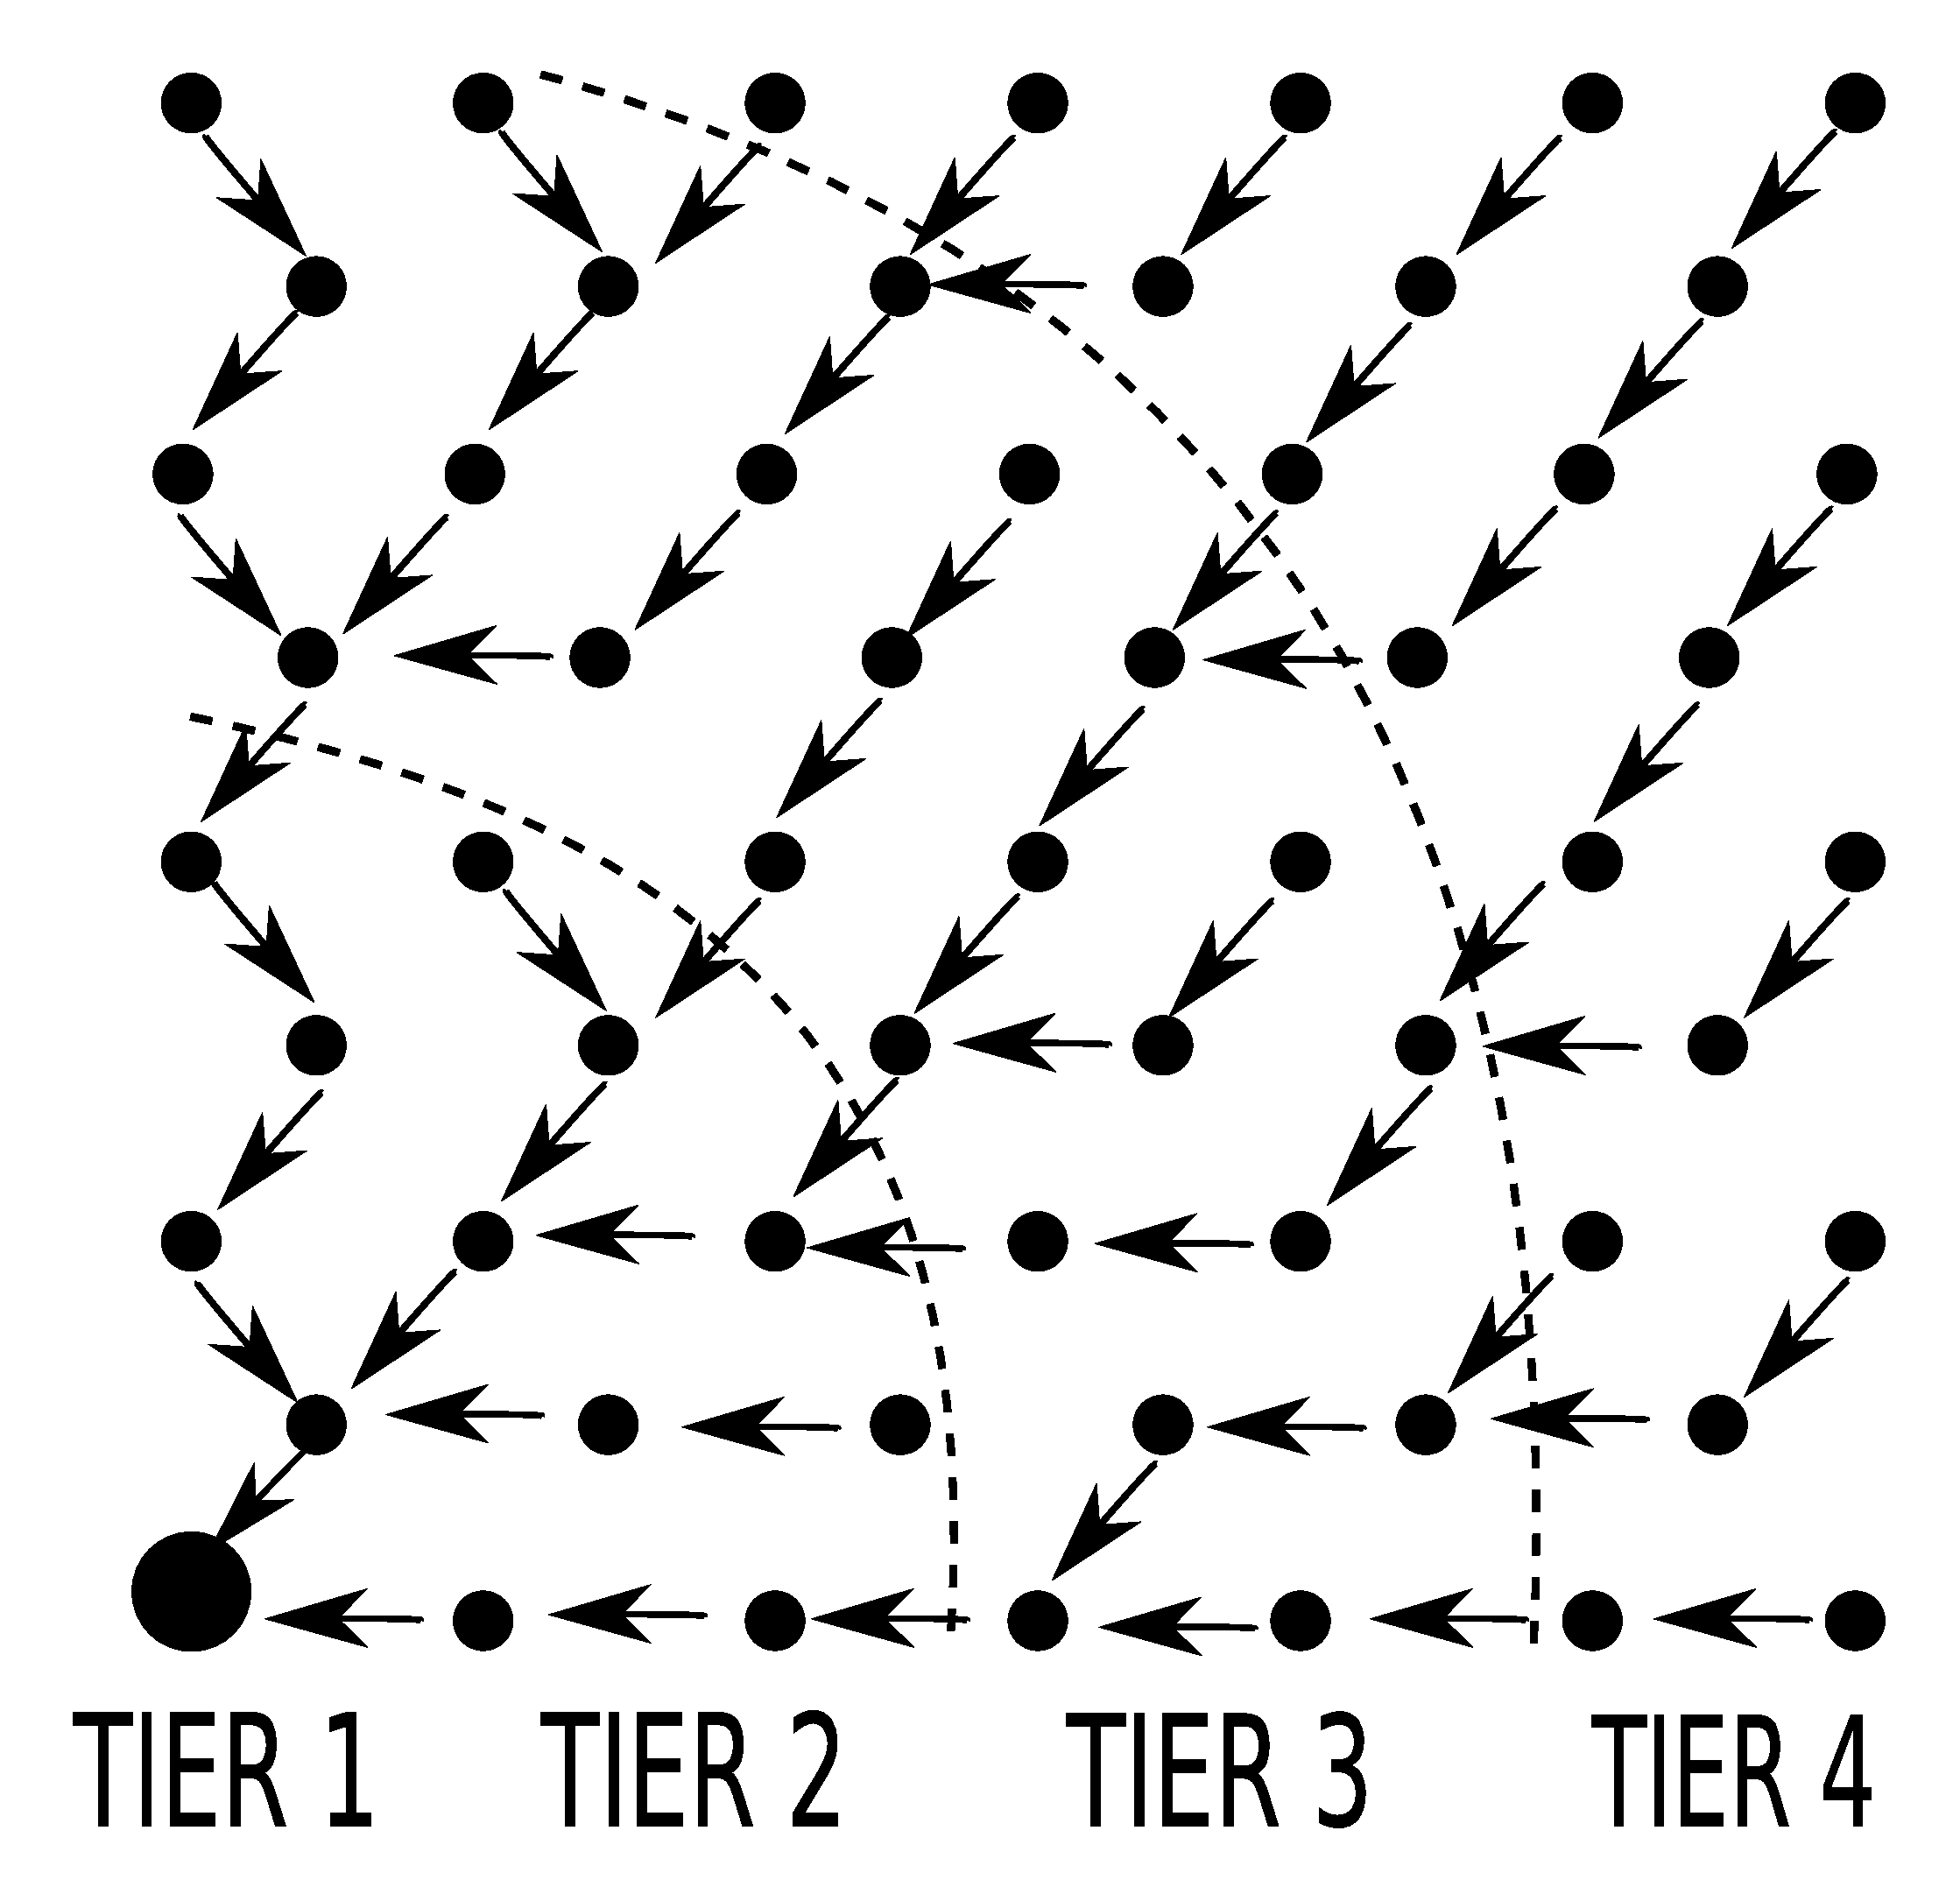
\includegraphics[width=2.5in]{fig/scenario_2a}
	\caption{Sensor network that establishes a multi-tiered tree
	topology, where data are propagated toward higher tiers (lower in
	id), and eventually reach a sink node. To optimize network
	performance, for example to lower power consumption, data may be
	aggregated or compressed to decrease the size of the transmitted
	messages.}
	\label{fig:scenarioa}
\end{figure}

\begin{figure}
\centering
	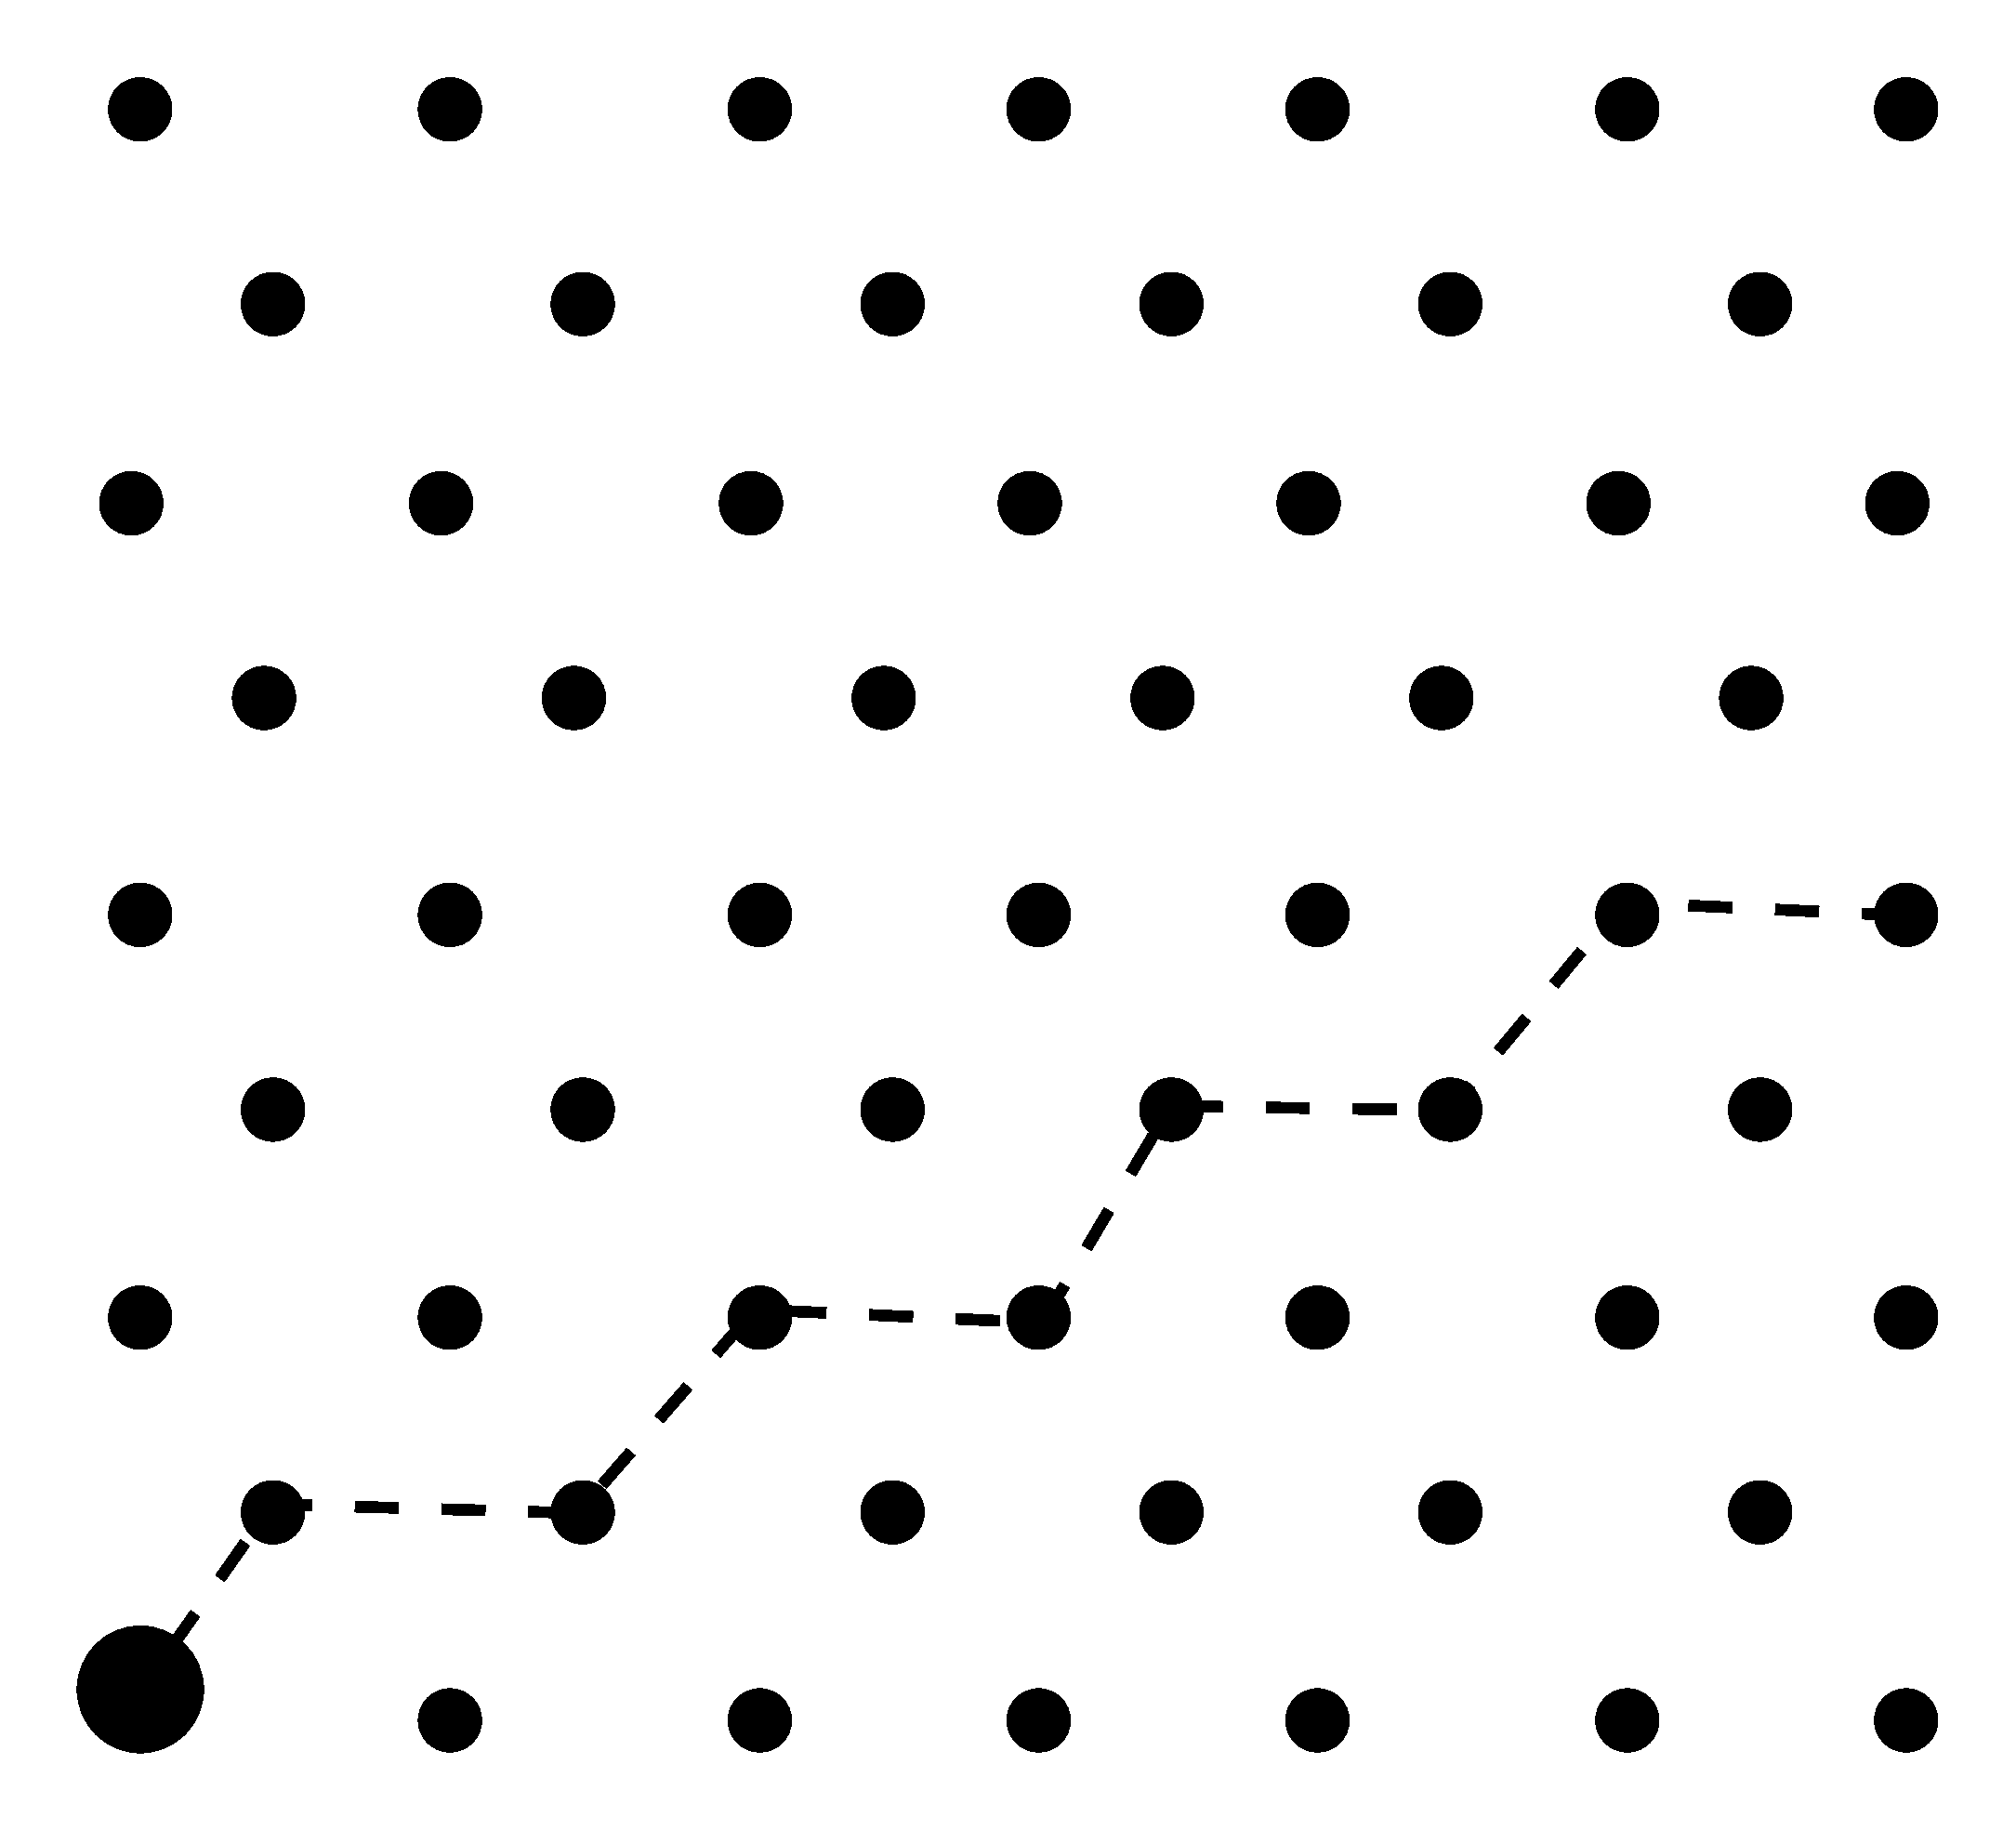
\includegraphics[width=2.5in]{fig/scenario_2b}
	\caption{In a result of some event, a point-to-point communication 
	between a node and the sink node is established. Network topology
	is flattened, no data aggregation is performed, and low delays are
	imported.}
	\label{fig:scenariob}
\end{figure}

Fennec Fox is a platform that provides the ability to have a reconfigurable
WSN that adapts to different application requirements. Through Swift Fox
we want to be able to program the Fennec Fox platform, seamlessly, in a
high-level and abstract fashion. Hence, Swift Fox is a simple policy-based 
programming language that specifies conditions that have to be meet for a
network to be reconfigured. Using the fire emergency application, we want
Swift Fox to reconfigure the network from the monitoring scenario to the
emergency scenario whenever light sensors show increased light intensity,
humidity sensors show decreased humidity, and temperature sensors show an
increase in temperature. Let \texttt{monitor} and \texttt{fire} represent
network state configurations that correspond to the two aforementioned
scenarios (\textit{i.e.,} the home monitoring environment and the fire
emergency response). Then, using Swift Fox language we would like to be
able to express a condition, represented by an event $e$ captured by
the sensors, which would trigger a transition on the network configuration 
from \texttt{monitor} state to \texttt{fire} state. 

\begin{figure}[htp]
\centering
        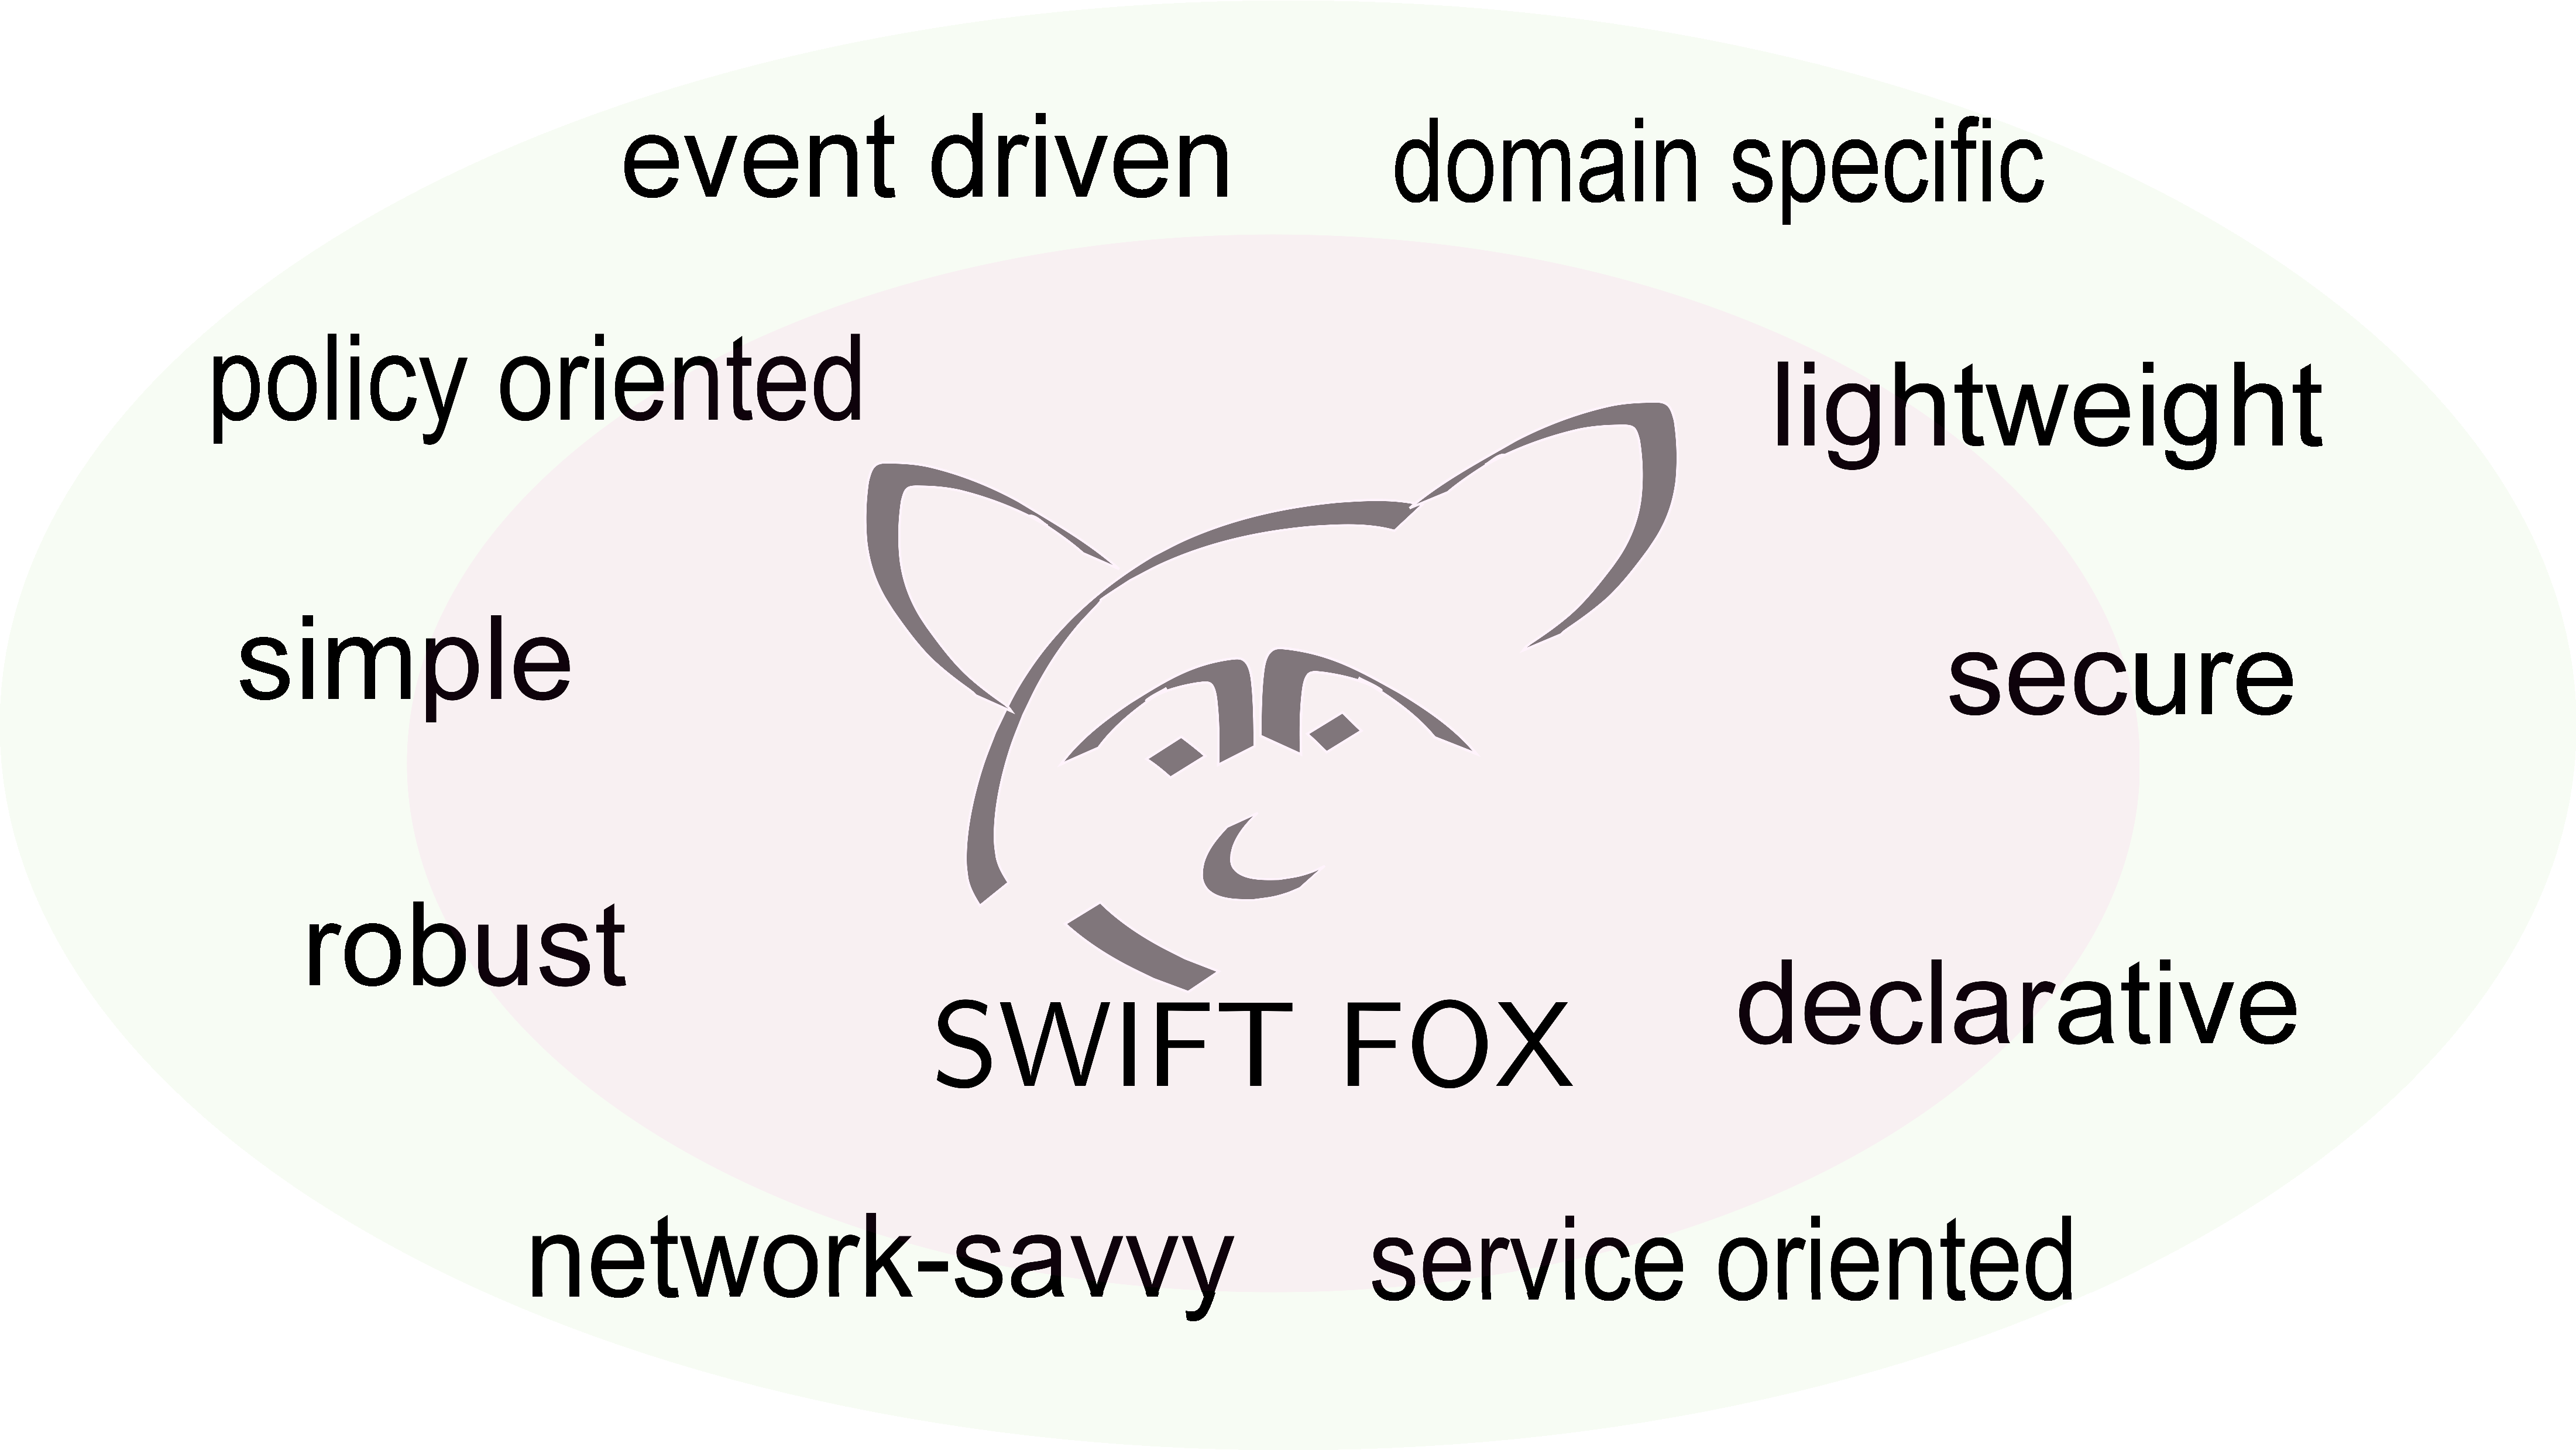
\includegraphics[scale=0.15]{fig/buzz.eps}
        \caption{Swift Fox buzzwords.}
        \label{fig:buzz}
\end{figure}

We define eleven objectives that Swift Fox should provide in order to
become a successful programming language and we specify them in a form of
``buzzwords''. These buzzwords were depicted on Figure \ref{fig:buzz}, and
are defined as follows:

\begin{enumerate}
	\item \textbf{Policy oriented}		\\
	\textit{Policies} describe precisely the behavior of entities
	that reside within the bounds of a \textit{policy domain}. Swift
	Fox allows, implicitly, the definition of a policy domain by
	giving the ability to describe, seamlessly and accurately,
	reconfiguration scenarios in an intuitive way. In general, each
	entity (\textit{i.e.,} a sensor node) is capable of responding
	differently to certain stimuli, based on the actual facilities
	provided by the underlying reconfiguration platform
	(\textit{i.e.,} Fennec Fox). For example, given the sensation of a
	certain event that indicates a critical incident, a node can cause
	the reconfiguration of the whole network in order to best
	disseminate critical data (\textit{e.g.,} proof of destruction
	or imminent hazard). Evidently, not all possible responses are
	permissible, either for security reasons (\textit{e.g.,} a node
	that does not have a vibration sensor should not be able to
	reconfigure the network for an earthquake response) or for
	application-specific purposes (\textit{e.g.,} there might be a
	strict priority among different applications based on their
	resource consumption). Through Swift Fox the task of defining a
	\textit{deterministic} and \textit{authoritative} behavior for the 
	WSN, as a whole, is largely simplified and becomes less
	error-prone. This is accomplished by adopting a policy-based
	notation that captures the essence of the \textit{environment
	semantics} as well as the entities' \textit{rights},
	\textit{prohibitions} and \textit{obligations}. 
	
	\item \textbf{Secure}			\\
	WSNs communicate and provide their services over the wireless
	medium. The open nature and the omnipresence of wireless signals,
	along with the lack of physical barriers in most WSN
	installations, leave a window of opportunity open for the
	proliferation of malicious behavior (\textit{i.e.,} either because
	WSNs provide an infiltration channel to a certain domain or
	because the WSN is the target itself). Therefore, protection
	against malevolent adversaries will most likely be mandatory in
	the near future. Authentication protocols, access control
	mechanisms, and encryption schemes have been studied in the past
	(in the WSN context) and have already lead to established
	techniques that offer specific levels of \textit{assurance}.
	However, most of the available solutions are highly optimized for 
	certain scenarios. Hence, it is of paramount importance to allow 
	dynamic configurations that enable the reuse of \textit{trusted}, 
	mature, and provable-working security components. Swift Fox offers
	the potential for expressing, naturally, specific security
	guarantees as well as behavioral requirements for the WSN nodes.
	Moreover, it allows the combination of different security
	primitives (\textit{i.e.,} distributed authentication, key
	exchange, encryption) in a composable fashion that meet the needs 
	of the environment and serve the applications to the best extent
	possible.

	\item \textbf{Robust}			\\
	In Section \ref{sec:whitepaper_introduction}, we outlined some of the
	possible WSN usages and application scenarios. However, many
	of these tasks (\textit{e.g.,} battlefield surveillance, patient
	monitoring, inventory management) are critical because they might 
	either affect human lives or hinder assets that are essential for
	the efficient operation of other systems. In particular, for
	such tasks the WSN is not allowed to exhibit \textit{best-effort}
	behavior and it is considered a \textit{critical infrastructure}.
	Swift Fox provides \textit{error-resistant}, \textit{reliable}
	WSN configurations by allowing the deterministic expression of WSN
	states in a high-level fashion.	
	
	\item \textbf{Simple}			\\
	Swift Fox is designed to fuel the development of commercial WSN
	applications. Thus, we assume that the audience of the language,
	people that deploy WSNs or simple contractors, may not be aware of
	every underlying aspect of a WSN. Yet, Swift Fox should be able to
	provide a simple way of programming a WSN by defining
	reconfiguration policies.

        \item \textbf{Service Oriented}       \\
	Swift Fox provides a way to express stages in the lifetime of
	a WSN. Its service oriented architecture (SOA) is inherited
	from Fennec Fox platform, which provides network services for
	multiple applications. Swift Fox loosely integrates Fennec Fox
	services with their applications into a network program. This
	network program is a chain of network states, during which one
	application with its supporting network protocols is active, and
	transitions between network states occur in response to events
	sensed by the network.   

	\item \textbf{Declarative}		\\
	The management of WSNs requires well-defined declarative languages
	\cite{hug90}. The programmer should be able to describe
	\textit{what} should the network configuration be in every case,
	via event handling actions. In contrast to a procedural language 
	(like C), where the program is a set of step-by-step instructions
	for execution, a declarative language aims at providing assertions 
	on beginning conditions and destination targets
	\cite{jinghuang:online}. Nevertheless, like any programming
	language, it must be \textit{expressive} enough so both the
	programmer and the compiler to be able to grasp how the program
	performs over time.

	\item \textbf{Domain specific}		\\
	Swift Fox is designed specifically for programming and managing
	WSNs. Its usage scope is well defined for the middle layer of
	network management. Our language belongs to the same range of
	domain specific languages (DSLs), in the WSN context, like nesC and
	Verilog. In fact, at the moment of writing, nesC is the underlying 
	language that Swift Fox compiles into. As a DSL, Swift Fox is
	developed to address the needs of a given domain and therefore it
	can only cater to a limited number of concepts. This leads to a
	higher level language that improves the developers'
	\textit{productivity} and \textit{communication} with domain
	experts \cite{johan:online}. The typical characteristics of a
	domain specific language are the following: it is designed for a
	particular problem domain (in our case WSNs), it is intended to
	glue together with other languages to complete a system
	(\textit{e.g.,} nesC), and finally it resembles configuration code 
	(\textit{i.e.,} policy specifications) \cite{mfowler:online}.
	Moreover, keeping the language confined allows for use of
	libraries, which are pre-compiled in whatever languages they need,
	in order to complete the desired underlying tasks. The
	configuration part of the language can be \textit{expressive} and
	easily \textit{readable}. 

	\item \textbf{Lightweight}		\\
	Software subsystems can often be designed and implemented in a
	\textit{clear}, \textit{succinct}, and \textit{aesthetically
	pleasing} way, by using specialized linguistic formalisms. In cases
	where such formalisms are not compatible with the principal
	implementation language (\textit{e.g.,} nesC), lightweight
	languages \cite{dspinellis:1997} are necessary so as to provide the
	required primitives as meta-constructs. The minimalistic syntax of
	Swift Fox not only allows memory-efficient objective code, but also
	provides the ability to exploit the primitives of the underlying
	platform in an clear, straightforward, and coherent manner.

	\item \textbf{Network-savvy}		\\
	Swift Fox provides a computing abstraction for the TinyOS
	system and Fennec Fox platform, which contain libraries of various 
	protocols, such as medium access protocols (MAC), network protocols
	(\textit{e.g.,} TCP/IP \cite{dunkels:2003} and IPv6
	\cite{durvy:2008}), data dissemination protocols (\textit{e.g.,}
	Trickle\cite{levis:2004}), quality of information (QoI) protocols, 
	reconfiguration schemes (\textit{e.g.,} TENET \cite{gnawali:2006}
	and Mate \cite{levis:2002}), and on demand sensor addressing
	\cite{schurgers:2002}. Swift Fox allows the programmer to
	adequately match the services provided by various protocols to
	quality of service (QoS) expectations imposed by applications.

	\item \textbf{Platform independent}	\\
	Swift Fox compiles into nesC \cite{gay:2003} that is suported 
	by the Fennec Fox platform running on top of TinyOS. In some way,
	this approach resembles Java; Java code  is compiled into byte code
	for Java Virtual Machine (JVM). The same way as Java becomes
	platform independent through JVM, Swift Fox becomes independent
	through Fennec Fox. Currently, Fennec Fox supports only TinyOS;
	however, in future other popular embedded systems are expected to
	be supported, particularly Linux, and Contiki \cite{dunkels:2004a},
	which have strong commercial support. Other operating systems,
	such as MANTIS \cite{bhatti:2005}, LiteOS \cite{cao:2008}, SOS
	\cite{han:2005}, and Pixie OS \cite{lorincz:2008} will be supported
	as time will allow. Today, wireless sensor nodes running all these 
	operating systems create separate networks, with different
	programming environments, and with various programming interfaces.
	Swift Fox establishes a single application programming interface
	and unifies various, currently, disjointed network environments.
	Moreover, it greatly simplifies WSN deployment and management, and 
	encourages WSN production and deployment from various vendors.  

	\item \textbf{Event-driven}		\\
	Swift Fox belongs to a family of languages that express system
	policies, and compiles into the nesC language \cite{gay:2003}, a
	component-based event-driven programming language. The event-driven
	nature of sensors becomes more evident as hardware reconfiguration
	mechanisms get to be incorporated in the sensor nodes
	\cite{kateeb:2009}. The event-driven nature of Swift Fox stems from
	the \textit{event-condition-action} (ECA) information model of
	polices, which for the first time proposed and implemented in Bell 
	Labs in 1999, and called Policy Description Language (PLD)
	\cite{Lobo:1999:PDL:315149.315308}. As shown in PLD, this
	information model of policies allows the creation of a programing
	language that does not have to be based on any graphical
	representation (\textit{e.g.,} in Unified Modeling Language (UML)).
	Finally, Swift-Fox establishes a relation between the event-driven
	specification of an embedded system and the event-driven policy
	that describes WSNs reconfiguration.
\end{enumerate}


\section{Language Overview}

Swift-Fox like many other languages, such as AWK, ``was born from necessity
to meet a need'' \cite{aho:2008}. Similarly to AWK, we are aiming for a
simple language that we can easily use to express transitions between the
states of a WSN platform. These transitions occur in response to events
detected by the sensor nodes. Here we propose a simple
\textit{event-condition-action} language -- Swift Fox -- that we hope
will meet our expectations. Because we believe that we are the first one to
address the wireless sensor network reconfiguration problem by designing
a new programming language, we hope this language will become successful
outside the walls of the classroom. To make this a successful case, we
defined eleven characteristics which we want our language to posses: policy
oriented, secure, robust, simple, declarative, service oriented, 
domain specific, light weight, network savvy, platform independent, 
and event driven.

